\vspace{.3in}  %to enter vertical space
\subsection*{Draw some basic}
\begin{enumerate}
\vspace{.25in}
\item{\textbf{Draw a Point:}
      \begin{enumerate}
      \item{Goto to toolbar, click on \textbf{Point} icon 
\includegraphics[width=20px]{./images/point.png}}
      \item{Click on Drawing area where you want to create point.}
      \end{enumerate}}
%
\vspace{.25in}
\item{\textbf{Draw a Line:}
      \begin{enumerate}
      \item{Goto to toolbar, click on \textbf{Line} icon 
\includegraphics[width=20px]{./images/line.png}}
      \item{A nested toolbar opens, which show you different functions for creating a line. Choose the \textbf{Line with two points }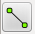
\includegraphics[width=20px]{./images/line2p.png}}
      \item{Select first point on drawing area}
      \item{Select second point on Drawing area}  
      \end{enumerate}}
%
\vspace{.25in}
\item{\textbf{Draw a Arc}
    \begin{enumerate}
    \item{Goto to toolbar, click on \textbf{Arc} icon
\includegraphics[width=20px]{./images/arc.png}}
    \item{A nested toolbar opens, which show you different functions for creating an arc. Choose the \textbf{Arc with center, point, Angles }
\includegraphics[width=20px]{./images/arc_cpa.png}}
    \item{Specify a point on Drawing area as a center of an arc. Hold the left click and move your cursor. You will see a preciew of circle as you move your cursor. Left click to unhold the cursor.}
    \item{Select two points: first point as your Starting point of Arc and second point as your End point of Arc.} 
    \end{enumerate}}
%
\vspace{.25in}    
\item{\textbf{Draw a Circle}\begin{enumerate}
    \item{Goto to toolbar, click on \textbf{Circle} icon
\includegraphics[width=20px]{./images/circle.png}}
    \item{A nested toolbar opens, which show you different functions for creating an Circle. Choose the \textbf{Circle with center, point }
\includegraphics[width=20px]{./images/circle_cp.png}}
    \item{Specify a point on Drawing area as a center of an arc. Hold the left click and move your cursor. You will see a preciew of circle as you move your cursor. Left click to unhold the cursor.}\end{enumerate}}
%
\vspace{.25in}
\item{\textbf{Draw a Ellipses}\begin{enumerate}
    \item{Goto to toolbar, click on \textbf{Ellipses} icon
\includegraphics[width=20px]{./images/ellipse.png}}
    \item{A nested toolbar opens, which show you different functions for creating an Ellipses. Choose the \textbf{Ellipse with center and 2 points }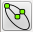
\includegraphics[width=20px]{./images/ellipse_c2p.png}}
    \item{Specify a point on Drawing area as a center of an arc. Hold the left click and move your cursor. You will see a preciew of ellipse as you move your cursor. Left click to unhold the cursor.}\end{enumerate}}
%
\vspace{.25in}
\item{\textbf{Draw a Polyline}
    \begin{enumerate}
    \item{Goto to toolbar, click on \textbf{Polyline} icon 
\includegraphics[width=20px]{./images/polyline.png}}
    \item{A nested toolbar opens, which show you different functions for creating an Polyline. Choose the \textbf{Create Polyline}
\includegraphics[width=20px]{./images/create_polyline.png}}
    \item{Click on one point on drawin are and then second point and then third...and so on till you want. To come out of this command, use Right click}
    \end{enumerate}}
%
\vspace{.25in}
\item{\textbf{Draw a Spline}\begin{enumerate}
    \item{Goto to toolbar, click on \textbf{Spline} icon 
\includegraphics[width=20px]{./images/spline.png}}
    \item{Define the points to which Spline go through. To come out of this command, use Right click}\end{enumerate}}
%
\vspace{.25in}
\item{\textbf{Draw a Text}\begin{enumerate}
    \item{Goto to toolbar, click on \textbf{Text} icon 
\includegraphics[width=20px]{./images/text.png}}
    \item{A dialog box will appear. Write the text you want on Dialog box and Set your text's font size and style. Then click on OK button
    \begin{figure}[h!] \centering 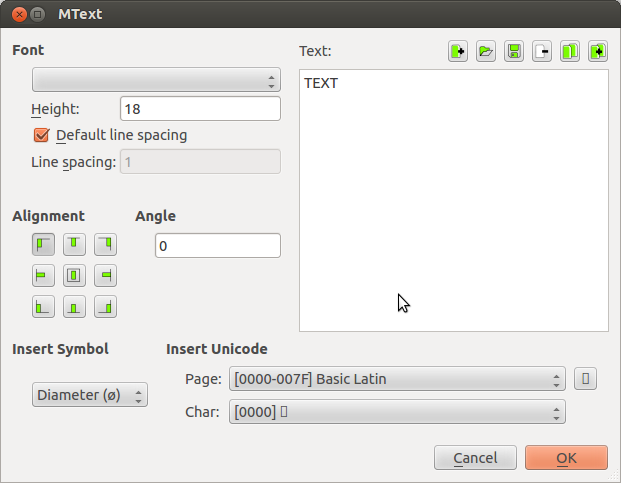
\includegraphics[width=200px]{./images/text_set.png} \end{figure}}
    \item{Specify the point on Drawing Area where you want to place your Text.}
    \end{enumerate}}
%
\vspace{.25in}
\item{\textbf{Draw a Image}\begin{enumerate}
    \item{Goto to toolbar, click on \textbf{Image} icon 
\includegraphics[width=20px]{./images/image.png}}
    \item{Select a image you want by browsing the images from your system}
    \item{select the point on drawing area where you want to place your image.}\end{enumerate}}
    %
\vspace{.25in}
\item{\textbf{Draw a Hatch}\begin{enumerate}
    \item{Goto to toolbar, click on \textbf{Text} icon 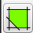
\includegraphics[width=20px]{./images/hatch.png}}
    \item{Select the closed entity which you want to hatch.}
    \item{ click on run button 
\includegraphics[height=20px]{./images/run.png}}
    \item{A dialog box will be opened, select the type of hatch and set the angle, and then click OK button.}
    \end{enumerate}}
\end{enumerate}
